%!TEX root = ../lections.tex
В 1834 году шотландский инженер-кораблестроитель и ученый Дж. Рассел, наблюдая за движением баржи по каналу, которую тащила пара лошадей, обратил внимание на удивительное явление. 

При внезапной остановке судна масса воды вокруг баржи в узком канале не остановилась, а собралась около носа судна, и затем оторвалась от него и в виде большого уединенного водного холма стала двигаться со скоростью около 8 миль в час. 

Удивительно, что форма холма в процессе его движения практически не менялась. Рассел назвал это движущееся по поверхности воды образование <<great solitary wave>>, что в переводе означает <<большая уединенная волна>>.	

Экспериментально получить явление, увиденное Расселом, можно следующим образом. Берется узкий, достаточно длинный бассейн, разделённый перегородкой:  
\begin{figure}[H]
	\centering
	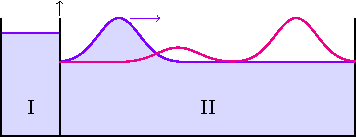
\includegraphics[scale=1.5]{img/soliton/pool}
\end{figure}
Подбирается соотношение масс воды в емкостях, при этом в части I уровень всегда должен быть выше. Резко поднимают задвижку, и, в зависимости от соотношения масс воды, могут побежать разные волны: разное количество холмов. 

В 1985 году Кортевег и де Вриз написали уравнения, описывающие явление, обнаруженное Расселом, и нашли форму волнового движения. Они рассматривали мелкий канал  со средней глубиной $l$, уровень воды $l+\eta(x,t)$, и получили следующее уравнение: 
\begin{equation*}
	\pdv{\eta}{t}=\frac32 \sqrt{\frac{g}{l}}\pdv{}{x}\qty(\frac32 \alpha \eta+\frac12 \eta^2+\frac13 \sigma \pdv[2]{\eta}{x}),
\end{equation*}
где $\sigma=\frac{l^3}{3}-\frac{Tl}{\rho g}$, $\alpha$ -- произвольная константа, $T$ -- коэффициент поверхностного натяжения, $\rho$ -- плотность жидкости.

В упрощённом виде это уравнение можно записать так:
\begin{equation}
	\pdv{u}{t}+u\pdv{u}{x}+\beta \pdv[3]{u}{x}=0.
	\label{eq:s3:1}
\end{equation}
Здесь $\beta$ -- некоторая константа, а последнее слагаемое характеризует дисперсию. Это уравнение простой волны, дополненное дисперсией. \textbf{Задание к  экзамену: построить дисперсионную характеристику}. 

\paragraph{Что дает дисперсия? } Рассмотрим квадратично-нелинейную среду без дисперсии.
Запустим в неё волну $e^{i(\omega_o t+kx)}$. Квадратичная среда порождает новые частоты: $\omega_0$ порождает $2\omega_0$. Если нет дисперсии, то нет пространственных масштабов, $2\omega_0$ порождает $3\omega_0$ и так далее, лавинным образом, спектр стремится в бесконечность. 
% \begin{figure}[H]
% 	\centering
% 	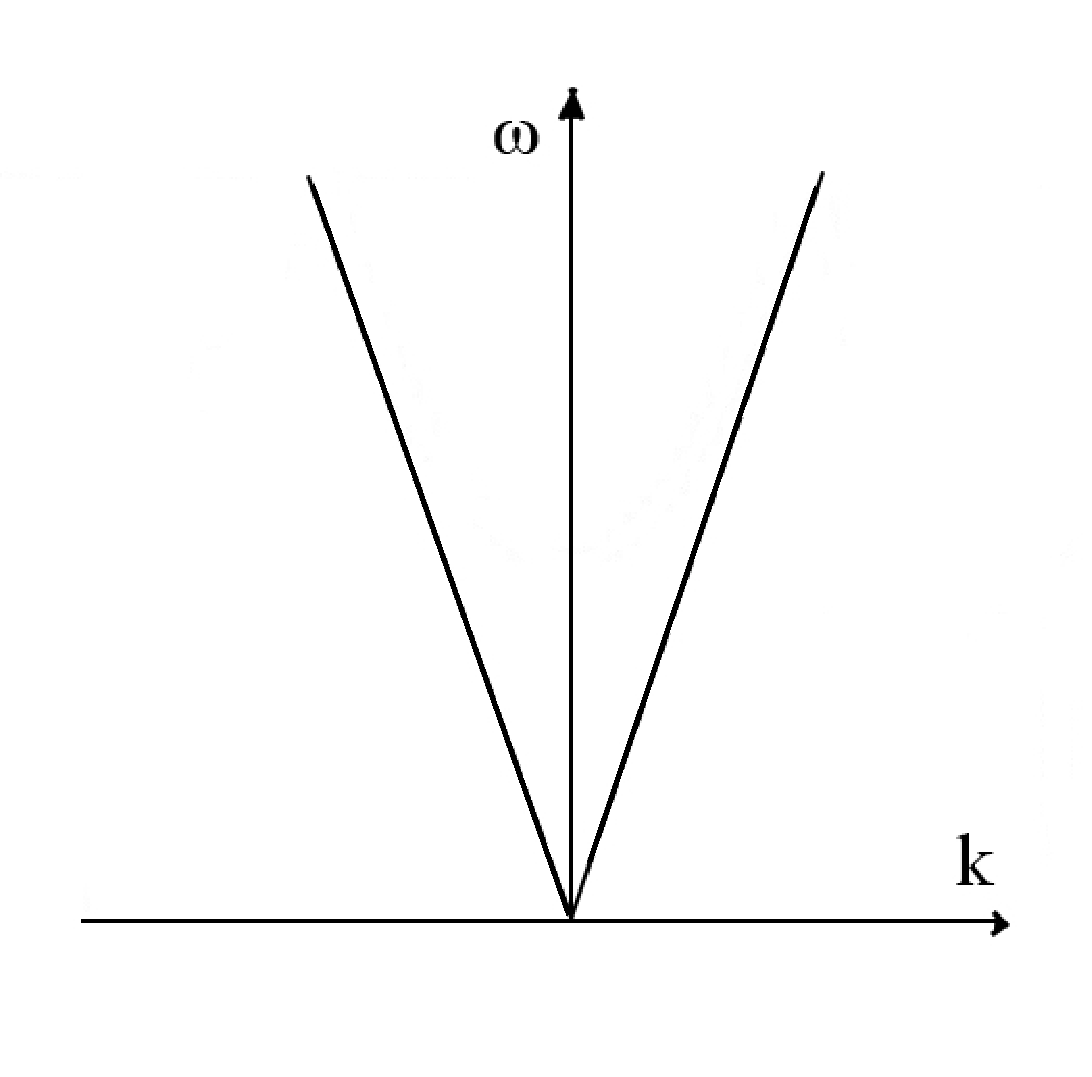
\includegraphics[width=0.4\linewidth]{fig/fig4.pdf}   
% \end{figure}

Слагаемое $\beta\pdv[3]{u}{x}$ даёт высокочастотную дисперсию, ограничивает ВЧ-спектр, стабилизирует решение и порождает солитон.
% Теперь включим дисперсию (в данном случае - высокочастотную). Она ограничивает частотный рост и стабилизирует волну. 

\paragraph{Решение задачи о солитоне. } Будем искать решение уравнения \eqref{eq:s3:1} в виде $u=u(x-Vt)=u(\xi)$, где $V=\const$:
\begin{equation}
	-\pdv{u}{\xi}+u\pdv{u}{\xi}+\beta \pdv[3]{u}{\xi}=0.
	\label{eq:s3:2}
\end{equation}
Один раз интегрируя, получим
\begin{equation}
	\beta \pdv[2]{u}{\xi}+\frac{u^2}{2}-Vu=0.
	\label{eq:s3:3}
\end{equation}
Это уравнение нелинейного осциллятора. Для простоты константу интегрирования приравняли  к нулю, что дает уровень, откуда изменяется $u(x,t)$. Запишем уравнение в виде системы
\begin{equation}
	\left\{\begin{aligned}
		&\dot{u}=y \\
		\beta &\dot{y} =Vu-\frac{u^2}{2}.		
	\end{aligned}\right.
	\label{eq:s3:4}
\end{equation}
% Получили систему для нелинейного осциллятора.
Можем найти потенциальную энергию, проинтегрировав правую часть второго уравнения системы \eqref{eq:s3:4}:
\begin{gather*}
	\beta \frac{y^2}{2}+E_{\text{п}} = \const
	\quad \Rightarrow \quad
	 E_{\text{п}} = \frac{u^3}{6}-V\frac{u^2}{2}
\end{gather*}
\begin{figure}[H]
	\centering
	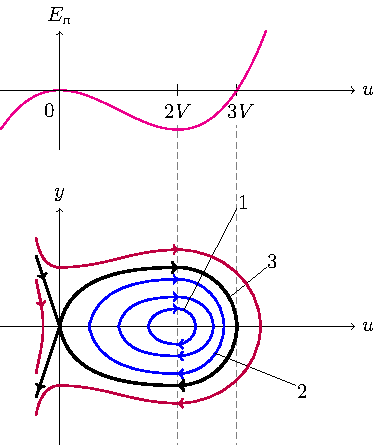
\includegraphics[scale=1.5]{img/soliton/phase_port_nonlin_osci}
	\caption{Фазовый портрет нелинейного осциллятора \eqref{eq:s3:4}}
	\label{fig:phase_port}
\end{figure}

% Фазовый портрет:
% \begin{figure}[H]
% 	\centering
% 	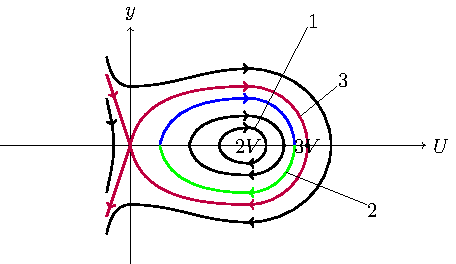
\includegraphics[width=0.5\linewidth]{fig/fig20.pdf}   
% \end{figure}
Математическим {образом солитона является гомоклиническая орбита} (траектория 3 на рисунке \ref{fig:phase_port}).

% 22.04

% Напомню, что дифференцирование в системе \eqref{eq:36} производится по бегущей координате. 

Вернемся к фазовому портрету. Неограниченные траектории лишены физического смысла, поэтому нас интересуют только ограниченные, то есть те, что находятся внутри петли сепаратрис, включая ее саму.

Возьмём траекторию вблизи состояния равновесия <<центр>> (на рисунке траектория 1). Она замкнутая, колебание близко к гармоническому. Колебание происходит на уровне $2V$. Таких колебаний континуум. 
\begin{figure}[H]
	\centering
	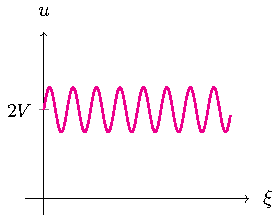
\includegraphics[scale=1.5]{img/soliton/2v}
\end{figure}

Выберем траекторию вблизи седла (на рисунке траектория 2), но все еще внутри гомоклинической орбиты. Выберем точку и положим при $\xi=0$ максимальную амплитуду. При движении по траектории к седлу (зеленым), u убывает. 
\begin{figure}[H]
	\centering
	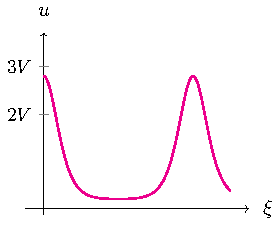
\includegraphics[scale=1.5]{img/soliton/25v}
\end{figure}

Около самого состояния равновесия скорость мала, движение в ее окрестности будет проходить медленно. В конце концов, при выходе из окрестности состояния равновесия, скорость опять увеличится. Мы получим профиль, так называемой, кноидальной волны, которая далека от гармонической. Волны такие из-за того, что система нелинейная. 

Если брать траектории все ближе к седлу, <<полка>> кноидального колебания будет увеличиваться. В конце концов, когда мы попадем на петлю:
\begin{figure}[H]
	\centering
	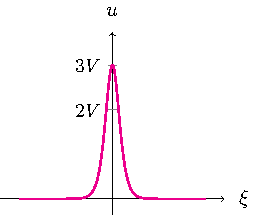
\includegraphics[scale=1.5]{img/soliton/3v}
\end{figure}
Для того, чтобы нарисовать профиль в области $\xi<0$, нужно пройти по траектории в обратном времени (время у нас $\xi$). Рисунок качественный, нарисован из понимания поведения функции на концах и знания максимальной амплитуды. 

Получившийся одиночный холм - это математический образ солитона.
% Точка 0 - решение, там нет пересечения траекторий, они стремятся туда асимптотически. 

\paragraph{Точный вид солитона.} Запишем уравнение \eqref{eq:s3:4} в виде одного:
\begin{equation}
	\beta\dv[2]{u}{\xi}=Vu-\frac{u^2}{2}
	\label{eq:s3:5}
\end{equation}
Решение будем искать в виде
\begin{equation}
	u=\frac{u_{max}}{\ch^2{(\xi / \Delta)}},
	\label{eq:s3:6}
\end{equation}
где введены параметры: $u_{max}, \Delta, V$ ($V$ скрыто в $\xi=x-Vt$). Подстановка \eqref{eq:s3:6} в \eqref{eq:s3:5} даёт
\begin{equation}
	\dv[2]{u}{\xi}=-2\frac{u_m}{\Delta^2}\frac{(3-2\ch^2{\xi / \Delta)}}{\ch^4{(\xi / \Delta)}}
	\label{eq:s3:7}
\end{equation}
\begin{gather*}
	\frac{2\beta u_m}{\Delta^2}\frac{(3-2\ch^2{(\xi / \Delta))}}{\ch^4{(\xi / \Delta)}}=\frac{u_m V}{\ch^2{(\xi / \Delta)}}-\frac{u_m^2}{2\ch^4{(\xi / \Delta)}}.
\end{gather*}
Приведя к общему знаменателю, получим
\begin{equation*}
	-2\beta[3-2\ch^2{(\xi / \Delta)}]=\Delta^2 \ch^2{(\xi / \Delta)}V-\frac{u_m \Delta^2}{2}
\end{equation*}
Чтобы это уравнение было тождеством, необходимо выполнение двух условий:
% Знаменатель не обращается в ноль.
\begin{equation}
	-6\beta=\frac{u_m \Delta^2}{2}
	\quad \Rightarrow \quad
	u_m \Delta^2= 12\beta,
	\label{eq:s3:8}
\end{equation}
\begin{equation}
	4\beta=\Delta^2V.
	\quad \Rightarrow \quad
	\Delta^2V=4\beta.
	\label{eq:s3:9}
\end{equation}
Параметры связаны, но их 3, а условия 2. Задав один, два других найдутся из \eqref{eq:s3:8} и \eqref{eq:s3:9}. 

$\beta$ характеризует дисперсию и не относится к самому солитону. $V$ -- скорость солитона, $u_m$ -- его высота, $\Delta$ оказывается шириной. Ширина солитона вычисляется на уровне $u=\frac{4u_m}{2+e}$. 
Из уравнения \eqref{eq:s3:9} следует, что, чем шире солитон, тем меньше его скорость, а из \eqref{eq:s3:8}, что чем шире солитон, тем меньше его амплитуда: $u_m=\frac{12\beta}{\Delta^2}$.

$V$ может принимать любые значения: это следствие непрерывности модели.

Если в диссипативной системе есть петля, то при изменении параметров она разрушается. Есть всего одна траектория, формирующая солитон. Солитоны столь интересны, потому что они устойчивы относительно большого числа начальных распределений. 


\subsection{Устойчивость солитона}
Рассмотрим стационарное уравнение Шрёдингера для определения статистического состояния. 
\begin{equation}
	\dv[2]{\psi}{x}+[u(x)+\epsilon]\psi=0.
	\label{eq:s3:10}
\end{equation}
Пусть $u(x)>0, ~u\rightarrow 0$ при $x\rightarrow \pm \infty$. Тогда, как известно из квантовой механики, есть решение дискретного спектра: $\epsilon=\epsilon_n$, $\psi, \psi' \rightarrow 0$ при $x\rightarrow \pm \infty$.\

Оказывается, существует связь между \eqref{eq:s3:10} и устойчивостью солитонов уравнения Кортевега -- де Фриза. Надо подставить нормированное решение:
\begin{equation*}
	\dv[2]{\psi}{x}+\qty[\frac{1}{6\beta}u(x,t)+\epsilon]\psi=0.
\end{equation*}
Покажем, что в случае солитона $\epsilon$ не будет зависеть от $t$.
\begin{equation*}
	u(x,t)=-6\beta\qty(\frac{\psi''}{\psi}+\epsilon),
\end{equation*}
где штрихом обозначено дифференцирование по $x$. Подставим такое решение в уравнение Кортевега - де Фриза:
\begin{equation}
	\pdv{u}{t}+u\pdv{u}{x}+\beta \pdv[3]{u}{x}=0.
	\quad\Rightarrow\quad
	\psi^2\dv{\epsilon}{t}=(\psi'A-A\psi'), \quad \text{где}
	\label{eq:s3:11}
\end{equation}
\begin{equation*}
	A(x,t)=6\beta\qty(\frac1{\beta}\pdv{\psi}{t}-3\frac{\psi'\psi''}{\psi}+\psi'''-\frac{\epsilon}{6}\psi').
\end{equation*}

Проинтегрируем \eqref{eq:s3:11} по переменной $x$ в бесконечных пределах. Вспомним, что $\psi, \psi' \rightarrow 0$ при $x\rightarrow \pm \infty$. Получим:
\begin{equation*}
	\dv{\epsilon}{t}\int^{+\infty}_{-\infty}\psi^2dx=0.
\end{equation*}

В силу нормировки интеграл не равен нулю. Следовательно, $\dv{\epsilon}{t}=0$ и $\epsilon\neq \epsilon(t)$.
Запишем ранее полученное уравнение солитона:
\begin{equation*}
	u(x,t)=u_{\max}\ch^{-2}\qty(\frac{x-Vt}{\Delta}).
\end{equation*}
Так как спектр $\epsilon$ не зависит от $t$, можем $t$ можно выбрать любое. Для удобства положим $t=0$, тогда уравнение \eqref{eq:s3:10} примет вид
\begin{equation}
	\psi''+(u_0 \ch^{-2}\alpha x+\epsilon)\psi=0, \qq{где}
	u_0=\frac{u_m}{6\beta},\quad \alpha=\frac1{\Delta}.
	\label{eq:s3:12}
\end{equation}

Такая задача решена в III томе Ландау\footnote{Параграф 23, задача 4}, и там показано следующее:
\begin{equation*}
	\epsilon_n=-\alpha(s-n), \quad
		n=0,1,2,\ldots; \quad n<s,
\end{equation*}
где $s=\frac12\qty(-1+\sqrt{1+\frac{4u_0}{\alpha^2}})$. Подставив $u_0$ и $\alpha$ в выражение для $s$, а затем применив формулы \eqref{eq:s3:8} и \eqref{eq:s3:9}, получим
\begin{equation*}
	s=\frac12\qty(-1+\sqrt{\frac{4u_m\Delta^2}{6\beta}})=\frac12(-1+3)=1
\end{equation*}
Отсюда следует, что $\epsilon_n=-\alpha(1-n)$. Но так как $n<s$, а $s=1$, то единственно возможное значение энергии
\begin{equation*}
 	\epsilon_0=-\alpha^2=-\frac{4u_m}{12\beta}.
\end{equation*} 
% \\ 
	%  \\ 
% \end{gather*}

Если в уравнение Шредингера подставить уравнение солитона, такому потенциалу соответствует одно собственное значение. 

\paragraph{Более широкая теорема (без доказательства).} \textit{Пусть в начальный момент $t=0$ есть распределение $u(x,0)=f(x)$, положительно определенное ($f(\pm\infty)=0$), но не совпадающее с солитоном.}

\textit{Тогда, подставив $u(x,0)$ в уравнение Шредингера и решив его, получим столько $\epsilon_j$, сколько солитонов может существовать при таких начальных условиях.}

Пусть, например, мы подставили начальное распределение и получили три значения $\epsilon_j$: $\epsilon_1$, $\epsilon_2$, $\epsilon_3$. Тогда в среде возможно три солитона:
% \begin{figure}[H]
% 	\centering
% 	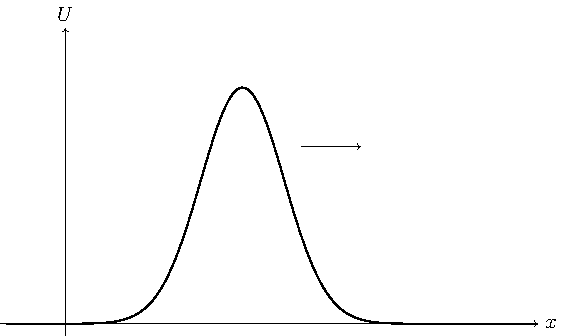
\includegraphics[width=0.4\linewidth]{fig/fig25.pdf}   
% \end{figure}

% Пусть $j=3$:
\begin{figure}[H]
	\centering
	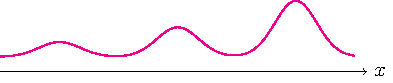
\includegraphics[scale=1.5]{img/soliton/solitons}
	\caption{Bound states}
\end{figure}
Такую задачу в квантовой механике называют <<обратной задачей рассеяния>>.

\paragraph{Качественные рассуждения. } Введем величину $\sigma=\frac{\Delta^2 u_m}{12 \beta}=1$. Здесь $u_m$ характеризует нелинейность, а $\beta$ - дисперсию. Предположим, что при $t=0$ задали такое распределение, что $\sigma \ll 1$. Это означает малость $u_m$, мы находимся около стационарного состояния (около нуля). 

Если мы близки к линейной задаче, главную роль играют дисперсионные механизмы. Есть области прозрачности и непрозрачности. В области прозрачности фазовая скорость у каждой компоненты своя. Пакет один -- и это солитон, и он расплывается.

Если же $\sigma \gg 1$, преобладает нелинейность. Она порождает новые гармоники: следует ожидать состава из солитонов. Дисперсия ограничивает частоты, фронт стабилизируется. Среда стабилизирует $\sigma$ к 1.
